%%%%%%%%%%%%%%%%%%%%%%%%%%%%%%%%%%%%%%%%%%%%%%%%%%%%%%%%%%%%%%%%%%%%%%%%%%%%%%%%
%% Plantilla de memoria en LaTeX para la ETSIT - Universidad Rey Juan Carlos
%%
%% Por Gregorio Robles <grex arroba gsyc.urjc.es>
%%     Grupo de Sistemas y Comunicaciones
%%     Escuela Técnica Superior de Ingenieros de Telecomunicación
%%     Universidad Rey Juan Carlos
%% (muchas ideas tomadas de Internet, colegas del GSyC, antiguos alumnos...
%%  etc. Muchas gracias a todos)
%%
%% La última versión de esta plantilla está siempre disponible en:
%%     https://github.com/gregoriorobles/plantilla-memoria
%%
%% Para obtener PDF, ejecuta en la shell:
%%   make
%% (las imágenes deben ir en PNG o JPG)

%%%%%%%%%%%%%%%%%%%%%%%%%%%%%%%%%%%%%%%%%%%%%%%%%%%%%%%%%%%%%%%%%%%%%%%%%%%%%%%%

\documentclass[a4paper, 12pt]{book}
%\usepackage[T1]{fontenc}

\usepackage[a4paper, left=2.5cm, right=2.5cm, top=3cm, bottom=3cm]{geometry}
\usepackage{times}
\usepackage[utf8]{inputenc}
\usepackage[spanish]{babel} % Comenta esta línea si tu memoria es en inglés
\usepackage{url}
%\usepackage[dvipdfm]{graphicx}
\usepackage{graphicx}
\usepackage{float}  %% H para posicionar figuras
\usepackage[nottoc, notlot, notlof, notindex]{tocbibind} %% Opciones de índice
\usepackage{latexsym}  %% Logo LaTeX

\title{Memoria del Proyecto}
\author{Nombre del autor}

\renewcommand{\baselinestretch}{1.5}  %% Interlineado

\begin{document}

\renewcommand{\refname}{Bibliografía}  %% Renombrando
\renewcommand{\appendixname}{Apéndice}

%%%%%%%%%%%%%%%%%%%%%%%%%%%%%%%%%%%%%%%%%%%%%%%%%%%%%%%%%%%%%%%%%%%%%%%%%%%%%%%%
% PORTADA

\begin{titlepage}
\begin{center}
\includegraphics[scale=0.8]{img/URJ_logo_Color_POS.png}

\vspace{1.75cm}

\Large
GRADO EN INGENIERIA EN SISTEMAS AUDIOVISUALES Y MULTIMEDIA

\vspace{0.4cm}

\large
Curso Académico 2020/2021

\vspace{0.8cm}

Trabajo Fin de Grado

\vspace{2.5cm}

\LARGE
IMPLEMENTACIÓN DE FUNCIONALIDADES EN LEARNINGML

\vspace{4cm}

\large
Autor : Isaac Merchán Blanco\\
Tutor : Dr. Gregorio Robles
\end{center}
\end{titlepage}

\newpage
\mbox{}
\thispagestyle{empty} % para que no se numere esta pagina


%%%%%%%%%%%%%%%%%%%%%%%%%%%%%%%%%%%%%%%%%%%%%%%%%%%%%%%%%%%%%%%%%%%%%%%%%%%%%%%%
%%%% Para firmar
\clearpage
\pagenumbering{gobble}
\chapter*{}

\vspace{-4cm}
\begin{center}
\LARGE
\textbf{Trabajo Fin de Grado}

\vspace{1cm}
\large
IMPLEMENTACIÓN DE FUNCIONALIDADES EN LEARNINGML

\vspace{1cm}
\large
\textbf{Autor :} Isaac Merchán Blanco \\
\textbf{Tutor :} Dr. Gregorio Robles

\end{center}

\vspace{1cm}
La defensa del presente Proyecto Fin de Carrera se realizó el día \qquad$\;\,$ de \qquad\qquad\qquad\qquad \newline de 2021, siendo calificada por el siguiente tribunal:


\vspace{0.5cm}
\textbf{Presidente:}

\vspace{1.2cm}
\textbf{Secretario:}

\vspace{1.2cm}
\textbf{Vocal:}


\vspace{1.2cm}
y habiendo obtenido la siguiente calificación:

\vspace{1cm}
\textbf{Calificación:}


\vspace{1cm}
\begin{flushright}
Fuenlabrada, a \qquad$\;\,$ de \qquad\qquad\qquad\qquad de 2021
\end{flushright}

%%%%%%%%%%%%%%%%%%%%%%%%%%%%%%%%%%%%%%%%%%%%%%%%%%%%%%%%%%%%%%%%%%%%%%%%%%%%%%%%
%%%% Dedicatoria

\chapter*{}
\pagenumbering{Roman} % para comenzar la numeracion de paginas en numeros romanos
\begin{flushright}
\textit{Dedicado a \\
mi familia y amigos}
\end{flushright}

%%%%%%%%%%%%%%%%%%%%%%%%%%%%%%%%%%%%%%%%%%%%%%%%%%%%%%%%%%%%%%%%%%%%%%%%%%%%%%%%
%%%% Agradecimientos

\chapter*{Agradecimientos}
%\addcontentsline{toc}{chapter}{Agradecimientos} % si queremos que aparezca en el índice
\markboth{AGRADECIMIENTOS}{AGRADECIMIENTOS} % encabezado 

Quiero agradecer a mis padres quienes han sido capaces de aguantar mis peores momentos durante esta carrera. A mi madre que desde pequeño siempre ha estado ayudandome con todo lo que he necesitado y confiando en mi. Y a mi padre que aunque no pase tanto tiempo con él me ha inculcado unos valores y una forma de ver la vida que me han llevado a ser quien soy a día de hoy.

Quería agradecer también a mis amigos por estar siempre dispuestos a sacar un rato para vernos y hablar, esos momentos de descanso también forman parte de esto y sin ellos nada sería lo mismo.

Gracias también a mis companeros con los que he pasado estos últimos años de mi vida y una etapa muy importante, sin ellos esto hubiera sido aún más difícil. Han hecho que las clases, las tardes de estudio, las prácticas y, en general, la carrera sea más divertida.

Por último, agredecer a Gregorio su manera de explicar y su disposición para ayudarme siempre que he necesitado algo y a Juanda por dejarme colaborar en su página.


%%%%%%%%%%%%%%%%%%%%%%%%%%%%%%%%%%%%%%%%%%%%%%%%%%%%%%%%%%%%%%%%%%%%%%%%%%%%%%%%
%%%% Resumen

\chapter*{Resumen}
%\addcontentsline{toc}{chapter}{Resumen} % si queremos que aparezca en el índice
\markboth{RESUMEN}{RESUMEN} % encabezado

Aquí viene un resumen del proyecto.
Ha de constar de tres o cuatro párrafos, donde se presente de manera clara y concisa de qué va el proyecto. 
Han de quedar respondidas las siguientes preguntas:

\begin{itemize}
  \item ¿De qué va este proyecto? ¿Cuál es su objetivo principal?
  \item ¿Cómo se ha realizado? ¿Qué tecnologías están involucradas?
  \item ¿En qué contexto se ha realizado el proyecto? ¿Es un proyecto dentro de un marco general?
\end{itemize}

Lo mejor es escribir el resumen al final.

%%%%%%%%%%%%%%%%%%%%%%%%%%%%%%%%%%%%%%%%%%%%%%%%%%%%%%%%%%%%%%%%%%%%%%%%%%%%%%%%
%%%% Resumen en inglés

\chapter*{Summary}
%\addcontentsline{toc}{chapter}{Summary} % si queremos que aparezca en el índice
\markboth{SUMMARY}{SUMMARY} % encabezado

Here comes a translation of the ``Resumen'' into English. 
Please, double check it for correct grammar and spelling.
As it is the translation of the ``Resumen'', which is supposed to be written at the end, this as well should be filled out just before submitting.


%%%%%%%%%%%%%%%%%%%%%%%%%%%%%%%%%%%%%%%%%%%%%%%%%%%%%%%%%%%%%%%%%%%%%%%%%%%%%%%%
%%%%%%%%%%%%%%%%%%%%%%%%%%%%%%%%%%%%%%%%%%%%%%%%%%%%%%%%%%%%%%%%%%%%%%%%%%%%%%%%
% ÍNDICES %
%%%%%%%%%%%%%%%%%%%%%%%%%%%%%%%%%%%%%%%%%%%%%%%%%%%%%%%%%%%%%%%%%%%%%%%%%%%%%%%%

% Las buenas noticias es que los índices se generan automáticamente.
% Lo único que tienes que hacer es elegir cuáles quieren que se generen,
% y comentar/descomentar esa instrucción de LaTeX.

%%%% Índice de contenidos
\tableofcontents 
%%%% Índice de figuras
\cleardoublepage
%\addcontentsline{toc}{chapter}{Lista de figuras} % para que aparezca en el indice de contenidos
\listoffigures % indice de figuras
%%%% Índice de tablas
%\cleardoublepage
%\addcontentsline{toc}{chapter}{Lista de tablas} % para que aparezca en el indice de contenidos
%\listoftables % indice de tablas


%%%%%%%%%%%%%%%%%%%%%%%%%%%%%%%%%%%%%%%%%%%%%%%%%%%%%%%%%%%%%%%%%%%%%%%%%%%%%%%%
%%%%%%%%%%%%%%%%%%%%%%%%%%%%%%%%%%%%%%%%%%%%%%%%%%%%%%%%%%%%%%%%%%%%%%%%%%%%%%%%
% INTRODUCCIÓN %
%%%%%%%%%%%%%%%%%%%%%%%%%%%%%%%%%%%%%%%%%%%%%%%%%%%%%%%%%%%%%%%%%%%%%%%%%%%%%%%%

\cleardoublepage
\chapter{Introducción}
\label{sec:intro} % etiqueta para poder referenciar luego en el texto con ~\ref{sec:intro}
\pagenumbering{arabic} % para empezar la numeración de página con números

Hoy en día vivimos en un mundo digital en el cual hay una cantidad inmensa de datos. La obtención de estos crece a un ritmo exponencial, solo en 2018 se generaron 33 zettabytes (un zettabyte equivale a 1.000 millones de terabytes) lo que equivale a 16.5 veces más que en 2009 ~\cite{webstatista}. A pesar de esto, solo somos capaces de procesar el 0.5 \% ~\cite{machinelearning} y ese porcentaje cada vez va a menos ya que no se incrementa de la misma forma la capacidad de obtención que de procesado. El principal problema de esto está en la complejidad y cantidad de los datos pues los humanos no somos capaces muchas veces de extraer información útil de esos datos. Esto ha hecho que se fomente el estudio de distintos campos, uno de ellos es el \emph{machine learning}. Estas limitaciones mencionadas anteriormente desaparecen en el momento en el cual el \emph{machine learning} entra en juego, ya que es capaz de procesar grandes cantidades de datos complejos y transformarlos en información legible y fácil de analizar por los los humanos.

El \emph{machine learning} (o aprendizaje automático) es la rama de la inteligencia artificial que trata de implementar el aprendizaje automático de máquinas a través de un entrenamiento. A pesar de ser un concepto relativamente nuevo, se basa en campos de estudio anteriores como la modelación estadística y o el reconocimiento de patrones.

\section{Presentación de la aplicación}
\label{sec:presentacionaplicacion}

Este Trabajo Fin de Grado tiene como principal objetivo la integración de los algortimos de aprendizaje automático de Naive Bayes y K-NN en la web de LearningML que actualmente solo utiliza el método de redes neuronales para clasficar imágenes o texto.

LearnignML es una web creada por Juan David Rodríguez García utilizando Angular y esta construida de tal manera que cualquier persona sin grandes conocimientos sobre el aprendizaje autmático pueda crear un modelo, entrenarlo y después probarlo. La web además permite descargar el modelo creado en un archivo JSON para después poder cargarlo sin necesidad de crearlo de nuevo, esto es muy útil ya que de esta manera no se tienen que volver a introducir todas las entradas para el aprendizaje, si no que directamente se puede importar un modelo creado previamente e introducir una entrada para ver su funcionamiento. También tiene la opcion de registrarse y poder guardar los modelos en tu cuenta o incluso tener proyectos compartidos entre varias personas. Por último, permite crear un modelo en Scratch y utilizarlo en la web aunque esta parte no se verá durante este trabajo.


\section{Estructura de la memoria}
\label{sec:estructura}

La memoria empieza con un resumen, en el que se explica brevemente en que consiste el proyecto, así como las tecnologias que se han usado para llevarlo a cabo. A continuación, se sitúan los agradecimiento y los índices, tanto el general como el de figuras. Finalmente, van los 6 capítulos en lo que se divide la memoria.

\begin{itemize}
  \item \textbf{Capítulo 1: Introducción.} En el primer capítulo se hace una breve explicación de en que consiste la web de LearningML y la estructura que va a seguir el trabajo.
  
  \item \textbf{Capítulo 2: Objetivos.} En este capítulo se describen los objetivos principales y específicos del trabajo y la planificación temporal de este.
  
  \item \textbf{Capítulo 3: Estado del arte.} Se trata de una breve explicación sobre la mayoría de las teconologías utilizadas en el desarrollo de la aplicación web.

  \item \textbf{Capítulo 4: Diseño e implementación.} Se desccribe de manera detallada tanto los cambios previos en la estructura como la arquitectura final de la web así como la implementación de los dos modelos de aprendizaje.
  
  \item \textbf{Capítulo 5: Experimentos y validación.} Se comprueba si funcionan correctamente las funcionalidades implementadas en la web de LearningML.
  
  \item \textbf{Capítulo 6: Conclusiones.} Por último, se repasa todo lo aprendido durante el desarrollo del proyecto y se comentan algunas mejoras o funciones que se podrían implementar en un futuro.
  
\end{itemize}



%%%%%%%%%%%%%%%%%%%%%%%%%%%%%%%%%%%%%%%%%%%%%%%%%%%%%%%%%%%%%%%%%%%%%%%%%%%%%%%%
%%%%%%%%%%%%%%%%%%%%%%%%%%%%%%%%%%%%%%%%%%%%%%%%%%%%%%%%%%%%%%%%%%%%%%%%%%%%%%%%
% OBJETIVOS %
%%%%%%%%%%%%%%%%%%%%%%%%%%%%%%%%%%%%%%%%%%%%%%%%%%%%%%%%%%%%%%%%%%%%%%%%%%%%%%%%

\cleardoublepage % empezamos en página impar
\chapter{Objetivos} % título del capítulo (se muestra)
\label{chap:objetivos} % identificador del capítulo (no se muestra, es para poder referenciarlo)

\section{Objetivo general} % título de sección (se muestra)
\label{sec:objetivo-general} % identificador de sección (no se muestra, es para poder referenciarla)

Mi trabajo fin de grado consiste en añadir los algortimos de aprendizaje automático de Bayes y K-NN de manera intuitiva e independientemente de si se quieren clasificar textos o imágenes a la web de LearningML.

\section{Objetivos específicos}
\label{sec:objetivos-especificos}

Para la realización del objetivo general se han planteado los siguientes objetivos específicos:
\begin{itemize}
  
	\item Reorganizar la manera de trabajar de LearningML para separar la obtención de datos del algorítmo utilizado.
 
	\item Implementar el algorítmo de Bayes y K-NN para que funcionen como dos clasificadores de tal forma que primero entrenen con las entradas de aprendizaje y luego evaluen otra entrada proporcionada por el usuario y la asigne correctamente a uno de los grupos creados previamente.
  
	\item Añadir en la interfaz una manera de poder elegir el tipo de algorítmo que se quiere utilizar de forma independiente a si los elementos a clasificar son texto o imágenes.

	\item Dejar que el usuario pueda tocar algunos de los parámetros de los clasificadores.

\end{itemize}


\section{Planificación temporal}
\label{sec:planificacion-temporal}

La primera idea que tuve de empezar con el Trabajo Fin de Grado (TFG) fue en Enero de 2021 y quería hacerlo a la vez que las prácticas entonces me puse en contacto con Gregorio y me comentó esto. Me llamo la atención la web de LearningML ya que recuerdo haber utilizado Scratch en el colegio y me parecía interesante aportar algo aunque sea de manera indirecta a que los niños se interesen por la programación.
En principio este proyecto iba a ser tanto prácticas como TFG y le iba a poder dedicar bastante horas todos los dias, sin embargo, me aceptaron en unas prácticas y no tuve tanto tiempo ya que estas eran de jornada completa. Además de esto, aun tenía una asignatura pendiente asi que era difícil establecer un horario concreto para dedicarle tiempo al proyecto. Cuando no tenía un examen cerca, al salir de trabajar me ponía con ello un rato y luego los fines de semana por la mañana también le dedicaba algo de tiempo. 
Recuerdo que primero tuve que aprender como funcionaba Angular y Typescript con un curso que tiene Juanda. Practicando y familiarizandome con la forma de trabajar en Angular.
Después tuve varias reuniones con Juanda (creador de LearningML) para ver como funcionaba la aplicacion de LearningML y donde había que añadir los cambios.
También tuve que buscar que librerias ya construidas de Bayes y K-NN podiamos adaptar para usarlas en la web y finalmente ponerme a ello. Para K-NN si que conseguí encontrar una librería que me sirvió aunque por como se obtienen los datos, había que procesarlos de nuevo antes de usarlos. Para Bayes no encontré nada y tuve que crear el clasificador desde cero lo que me llevo algo más de tiempo que en el otro caso.
Por último, quedaba la tarea de trasladar todo eso al papel. Me puse en contacto con mi tutor y enseguida me paso una plantilla con los apartados a rellenar y comencé a hacerlo hasta que finalmente, con no mucho tiempo de margen para entregar el trabajo, terminé.


%%%%%%%%%%%%%%%%%%%%%%%%%%%%%%%%%%%%%%%%%%%%%%%%%%%%%%%%%%%%%%%%%%%%%%%%%%%%%%%%
%%%%%%%%%%%%%%%%%%%%%%%%%%%%%%%%%%%%%%%%%%%%%%%%%%%%%%%%%%%%%%%%%%%%%%%%%%%%%%%%
% ESTADO DEL ARTE %
%%%%%%%%%%%%%%%%%%%%%%%%%%%%%%%%%%%%%%%%%%%%%%%%%%%%%%%%%%%%%%%%%%%%%%%%%%%%%%%%

\cleardoublepage
\chapter{Estado del arte}
\label{chap:estado}

En este apartado veremos tanto las tecnologias utilizadas como una breve explicación sobre lo que es el modelo de Bayes y de K-NN.

\section{HTML5} 
\label{sec:html5}

HTML ~\cite{htmlw3} ~\cite{htmlwhat} (HyperText Markup Language) es un lenguaje de marcado que se utiliza para describir la estructura de las páginas web. HTML5 es la quinta versión de este lenguaje. A lo largo de todas las versiones se han incorporado y eliminado diferentes características, con el fin de hacerlo más eficiente y facilitar el desarrollo web compatibles con distintos navegadores y plataformas, y manteniéndose también compatible con las versiones anteriores.
A pesar de ser un estándar a cargo del Consorcio WWW, fue la asociación WHATWG, formada por Apple, Opera y Mozilla, la que publicó el primer borrador de HTML5 cuando W3C decidió dejar de evolucionar HTML. Más tarde W3C y WHATWG trabajaron juntos durante varios años en el desarrollo de HTML5, hasta que se separaron debido a sus diferentes objetivos, W3C quería publicar una versión terminada mientras que WHATWG quería seguir trabajando, manteniendo HTML5 en constante evolución.
Algunas de las principales características de HTML5 son:
\begin{itemize}
	\item Incorpora nuevas etiquetas que especifican la semántica del contenido, ayudando a interpretar mejor la página. Antes solo teníamos \textless{}div\textgreater{} para definir cualquier sección, ahora podemos utilizar \textless{}header\textgreater{}, \textless{}nav\textgreater{}, \textless{}section\textgreater{}, \textless{}footer\textgreater{}, entre otros.

	\item Ofrece también mejoras en los formularios como validaciones, nuevos tipos de campos (email, date, range, etc) y nuevos atributos, por ejemplo, multiple, placeholder o form.

	\item Cuenta con numerosas APIs. Algunas de ellas son:

	\begin{itemize}

		\item Audio y video: permite incrustar elementos de audio y vídeo y reproducirlo desde el propio navegador.

		\item Web Storage: permite almacenar datos del lado del cliente, cuando la sesión está activa.

        	\item Canvas: que permite hacer dibujos, juegos, animaciones, etc.

		\item Geolocalización: permite mostrar e interactuar con un mapa de Google Maps.

	\end{itemize}
\end{itemize}

\section{TypeScript} 
\label{sec:typescript}

TypeScript~\cite{typescript} un lenguaje de programación, de código abierto y desarrollado por Microsoft.
Nació como una necesidad de mejorar algunos problemas de JavaScript, entre ellos el hecho de que es bastante complicado crear aplicaciones a gran escala con JavaScript. Está pensado para el desarrollo de aplicaciones robustas y escalables, y se puede utilizar tanto en el lado del cliente como en el del servidor junto a Node.js.

TypeScript es un superconjunto de JavaScript, es decir, se trata de un lenguaje creador a partir de JavaScript. Los programas de JavaScript son programas válidos de TypeScript. Esto permite integrar JavaScript en proyectos ya existentes, sin tener que rehacer todo el proyecto en TypeScript, ya que todo el código TypeScript se puede compilar en JavaScript nativo.
Las características más importantes de TypeScript son:

\begin{itemize}

	\item Tenemos a nuestra disposición las herramientas de JavaScript ES6 (Ecmascript 6). De esta forma se mantiene actualizado con las últimas mejoras de JavaScript.

	\item Cuenta con un tipado estático, por tanto, al crear variables podemos añadir el tipo de dato, así podemos evitar errores en tiempo de ejecución.

	\item Objetos basados en clases, lo cual hace más sencilla la programación orientada a objetos y añade más funcionalidad.

\end{itemize}

\section{Node.js} 
\label{sec:nodejs}

Node~\cite{nodejs} es un entorno de ejecución de JavaScript controlado por eventos asíncronos, diseñado para construir aplicaciones de red escalables.
Fue creado por Ryan Dahl en 2009 y está influenciado por algunos sistemas como Event Machine de Ruby ó Twisted de Python.

Cuando se utiliza JavaScript en el lado del cliente, es el navegador quien, a través de un programa interno (un motor), interpreta el código JavaScript. De este mismo modo, Node.js proporciona un entorno de ejecución JavaScript del lado del servidor, haciendo uso del motor V8 de Google, que se encarga de interpretar el código y ejecutarlo.
El motor V8 es el que Google usa en su navegador Chrome y es posible descargarlo e introducirlo en cualquier aplicación.

Node.js está pensado para soportar grandes cantidades de solicitudes muy altas gracias a su naturaleza asíncrona. El modelo de concurrencia más común está basado en la utilización de hilos del sistema operativo. Se genera un nuevo hilo para cada conexión, de modo que a mayor cantidad de personas, mayor cantidad de recursos consumidos del servidor y mayor número de servidores son necesarios. Node.js emplea un único hilo y un bucle de eventos asíncrono. Las nuevas peticiones son tratadas como eventos en este bucle,de esta forma, no se produce ningún tipo de bloqueo en el flujo de trabajo.

\section{Archivos JSON} 
\label{sec:archivosjson}

JSON (JavaScript Object Notation - Notación de Objetos de JavaScript) es un formato de intercambio de datos ~\cite{json}. Es sencillo tanto de escribir como de leer, lo que facilita que tanto los humanos como las máquinas sean capaces de utilizarlos y generarlos. Aunque esta basdo en un subconjunto del lenguaje de programación Javascript, es un formato de texto completamente independiente del lenguaje.

En el siguiente texto en formato JSON, podemos ver las dos estructuras que nos ofrece, una colección de pares de nombre/valor y una lista de valores. En el ejemplo, vemos que el tipo de clasificador será de texto en este caso y que dentro de los datos tendremos dos etiquetas, una de vocales con una lista de las entradas que pertenecen a esta etiqueta y otra de consonantes. 
{\footnotesize
\begin{verbatim}
{
    "type": "text",
    "data": {
        "vocales": [
            "aaa",
            "eee",
            "iii"
        ],
        "consonantes": [
            "sss",
            "ddd",
            "fff"
        ]
    }
}
\end{verbatim}
}

\section{Angular} 
\label{sec:angular}

Angular~\cite{angular} es un \emph{framework} de código abierto diseñado por Google. Permite crear aplicaciones web de una sola página, lo que se denomina SPA (Single Page Application). Utiliza TypeScript y HTML para el desarrollo de las aplicaciones web. 

Angular permite separar el \emph{frontend} del \emph{backend} y sigue un modelo MVC (Modelo-Vista-Controlador) el cual se verá como funciona en el siguiente apartado. De esta forma, las modificaciones y las actualizaciones de las aplicaciones son rápidas y sencillas. 

Una de las principales ventajas de este \emph{framework} y de las páginas SPA es la velocidad de carga entre las diferentes vistas de la aplicación. Cuando se cambia de vista no se recarga la página si no que éstas se cargan de manera dinámica, rápida y reactiva. 

Angular dispone de varias versiones, aportando todas ellas mejoras en dicho \emph{framework}. La primera versión de Angular, se conoce como AngularJS, y es la más distinta a las demás. El resto son actualizaciones de Angular 2. Cuando se definió la segunda versión se decidió modificar el nombre del \emph{framework} y dejarlo como Angular. La última versión estable es la versión 10, utilizada por LearningML.

La arquitectura de una aplicación Angular se basa en clases de 4 tipos distintos (módulos, componentes, servicios y directivas). Estas clases se identifican a través de decoradores, los cuales permiten cargar los metadatos necesarios que determinan a Angular como debe usar dichas clases.

\textbf{Módulos}.

Los módulos suministran el contexto de compilación de los componentes, es decir, es aquí donde se definen los diferentes componentes que van a formar la aplicación, las dependencias, las clases que actúan como servicios en la aplicación y las rutas de navegación que establecen las vistas de la aplicación. 

Toda aplicación angular tiene un módulo principal o raíz. Este módulo suele recibir el nombre de \emph{AppModule} y es el que inicia el sistema de arranque de la aplicación.

Al igual que en JavaScript, los módulos de Angular permiten importar y exportar funcionalidades proporcionadas por otros módulos, por lo que una aplicación puede tener más de un módulo, siendo cada uno de ellos independiente. La manera en que se organizan estos módulos ayuda a la creción de aplicaciones más complejas y a la reutilización de código. Además, permite que la carga inicial sea mínima, ya que cada módulo se carga a petición, es decir, cuando se va a utilizar. 

\textbf{Componentes}. 

Las aplicaciones Angular tienen un componente que es nexo de unión entre los diferentes componentes que forman la aplicación y el modelo de objeto del documento de la página (DOM). Los componentes son los que tienen la lógica y los datos de la aplicación. Son los que controlan las diferentes plantillas HTML que se cargan cuando se modifican las URLs. Estas plantillas HTML son las vistas que forman la interfaz de usuario.

De la misma forma que las aplicaciones diseñadas con Angular pueden tener más de un módulo, también pueden tener subcomponentes, que se pueden relacionar entre sí mediante dos tipos de vinculación de datos, eventos y propiedades. A través de los eventos, la aplicación responde a las entradas del usuario actualizando los datos. A través de las propiedades, se envían valores calculados de los datos de la aplicación a los HTMLs que forman las vistas. Esta vinculación de datos se puede producir en ambas direcciones, es decir, igual que los datos de la aplicación pueden modificar los HTMLs, los cambios en el DOM pueden modificar los datos de la aplicación.

El decorador @Component es el que determina que una clase actúe como un componente. 

\textbf{Servicios}

Los servicios son clases en las que se definen datos o funcionalidades generales que no están asociadas a una determinada vista. Son usados para compartir datos y operaciones entre componentes. También es donde se suele realizar toda la operativa de las peticiones a la API de las aplicaciones. Deben llevar el decorador @Injectable, pues es el que permite obtener los metadatos necesarios para que otras clases puedan inyectar sus dependencias. 

\textbf{Directivas}

Las directivas son clases en las que se definen los términos claves que se usan en las plantillas. Cuando se carga una vista, Angular procesa estos términos clave que modifican el HTML y el DOM de la aplicación. Por tanto, una plantilla, además de utilizar HTML para definir la vista, usa marcas propias de Angular que son estas directivas. 

Existen dos clases de directivas: (i) las de atributo, que modifican el comportamiento del componente, y (ii) las estructurales, que únicamente modifican la apariencia. 

Angular dispone de un enrutador, módulo que contiene un servicio para definir las rutas de navegación de la aplicación. Este módulo se ajusta a las convenciones de los navegadores. Es decir, tanto si se pone la URL en la barra de direcciones, como si se pincha un enlace en la aplicación, como si se hace \emph{click} en el botón de retroceso o avance, se carga a la página correspondiente. El enrutador es el que muestra u oculta una vista. Cada vez que se modifica la URL, el enrutador se encarga de añadir la ruta en el historial del navegador, es esto lo que permiete que los botones de retroceso y avance funcionen. Cada ruta de navegación está asociado a un componente. 

\subsection{MVC} 
\label{sec:mvc}

Las aplicaciones web se suelen desarrollar siguiendo una serie de pautas. El patrón que sigue Angular es el Modelo Vista Controlador (MVC), cuyos elementos son ~\cite{mvc} :

\begin{itemize}
  
	\item \textbf{Modelo:} es la representacion de los datos de toda la aplicación y, por tanto, maneja las consultas y todas las acciones relacionadas con base de datos en caso de que las hubiera. También tratará los datos para cumplir con las funcionalidades de la aplicacióon.
 
	\item \textbf{Vista:} recibe los datos y los sirve al usuario final en la interfaz. Ni el controlador ni el modelo se preocupan por el diseño ni la apariencia final, de todo el apartado visual eso se encargarán las vistas.

	\item \textbf{Controlador:} es el elemento principal, encargado de responder a las acciones de entrada y lanzar una serie de funciones asignadas previamente. Es decir, recibe un evento de entrada, se comunica con el modelo en caso de que sea necesario, consultan las vistas y responden al evento con una salida.

\end{itemize}

Las principales ventajas del MVC son las siguientes:

\begin{itemize}
  
	\item Mejora la escalabilidad, puesto que es un modelo sencillo en el que cada tipo de lógica esta separado.
 
	\item Facilita mantenimiento.

	\item Ofrece la posibilidad de reutilizar los componentes.

\end{itemize}

\subsection{Angular CLI} 
\label{sec:angularcli}

Angular CLI (Command Line Interface) ~\cite{articulobayes} es una herramienta de línea de instrucciones creada por el equipo de Angular. Es muy util a la hora de iniciar una aplicación web diseña con Angular, ya que con una sola instrucción, se genera el esqueleto de carpetas y archivos necesarios de la aplicación. Además, contiene herramientas predefinidas que ayudan al desarrollo y mantenimiento de este tipo de aplicaciones. Al crear una aplicación web con Angular CLI, dentro de la estructura de archivos, se crea un archivo de configuración, en el cual se añaden las dependencias necesarias para que la aplicación web compile y ejecute. Este archivo se va modificando conforme se van creando los componentes, servicios o directivas. Para ello, Angular CLI tiene instrucciones que permiten crear estas clases de manera sencilla, creando los distintos archivos que conforman un componente, un servicio o una directiva. Entre las herramientas predefinidas destaca el compilador, el sistema de testing y el servidor web.


También existe la posibilidad de poner notas al pie de página, por ejemplo, una para indicarte que visite la página del GSyC\footnote{\url{http://gsyc.es}}.

\section{TensorFlow} 
\label{sec:tensorflow}

TensorFlow ~\cite{tensorflow} es un sistema de aprendizaje automático de segunda generación creado por Google Brain y es la herramienta más utilizada en el mundo del Deep Learning. La decisión de liberar TensorFlow se tomó en noviembre de 2015, por lo que hoy es posible acceder a esta herramienta libremente y editarla en función de las necesidades. Esta biblitoeca, es una gran plataforma para construir y entrenar redes neuronales, que permiten detectar y descifrar patrones y correlaciones, similares al aprendizaje o razonamiento que usamos los humanos. 

\subsection{MobileNets} 
\label{sec:mobilenets}

MobileNets ~\cite{mobilenets} es, además de una librería de TensorFlow la cual vamos a utilizar, una red neuronal convolucional más eficiente ya que se basa en una capa convolucional normal, de la dimensión deseada, pero con un solo filtro. De esta manera, al pasar información por una capa se genera una sola convolución, que esta a su vez sirve como entrada a otra capa de convolución de tamaño fijo de filtro 1x1, con el número de filtros deseados en la convolución a sustituir.

Aunque todo esto suena bastante complejo, lo que a nosotros nos interesa es que vamos a usar esta librería para transformar las imágenes en vectores que serán las entradas del clasificador sin importar el tipo. Lo que haremos será quitar la última capa de la red neuronal que genera MobileNets y quedarnos con ese vector.

\section{Modelo de Naive Bayes} 
\label{sec:modelobayes}

El modelo de Naive Bayes ~\cite{articulobayes} consiste en un clasificador probabilístico bastante simple y que supone que las distintas características que se evalúan son independientes. Aunque esto no siempre es así, cuando evaluamos una gran cantidad de características, tiende a cumplirse. Esto es lo que simplifica en gran medida el clasificador y por lo que es muy utilizado cuando se necesitan procesar grandes dimensiones de datos y no se requiere demasiada exactitud. Este clasficador requiere unos datos de entrada de entrenamiento y cuantos más reciba, mejor funcionará. Además, el modelo de Naive Bayes es un modelo paramétrico, es decir, usa el conjunto de entrenamiento para aprender el modelo explícitamente. Lo que hace Naive Bayes es aprender de los datos de entrenamiento y luego predice la clase de la entrada de prueba con la mayor probabilidad a posteriori.

La fórmula de la probabilidad de una clase C dadas unas características desde F1 a Fn es la figura ~\ref{fig:formulabayes}.

\begin{figure}
	\centering
	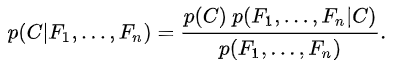
\includegraphics[width=9cm, keepaspectratio]{img/formulabayes}
	\caption{Fórmula de probabilidad de Naive Bayes.}
	\label{fig:formulabayes}
\end{figure}

En la práctica ~\cite{machinelearning} solo importa el numerador, puesto que el denominador no depende de C y los valores de Fi son datos, por lo que el denominador es constante en la práctica. En el numerador es donde se asume que cada Fi es independiente de cualquier otra Fj (siempre que j es distinta de i) cuando estas dependen de C. Esto significa que haciendo estos supuestos, la probabilidad de C teniendo en cuenta las variables clasificatorias puede expresarse como muestra la imágen ~\ref{fig:ffinalbayes} donde Z es un factor que depende unicamente de F1 \dots Fn, es decir, constante si los valores de Fi son conocidos.

\begin{figure}
	\centering
	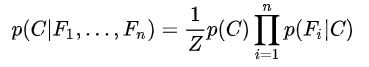
\includegraphics[width=9cm, keepaspectratio]{img/ffinalbayes}
	\caption{Fórmula de final de Naive Bayes.}\label{fig:ffinalbayes}
\end{figure}

Lo que hace el clasificador finalmente es calcular la probabilidad de cada posible clase con las características de entrada y asgina la entrada a esa clase.

\section{Modelo K-NN o K vecinos más cercanos} 
\label{sec:modeloknn}

El modelo de K-NN (\emph{k-nearest neighbors}) o \emph{k} vecinos más cercanos ~\cite{knn1} ~\cite{knn2} es un método estadístico de reconocimiento de patrones supervisado. Es un modelo no paramétrico ya que usa directamente los datos de entrenamiento para inferir cada vez la clasificación de una nueva entrada pero sin construir explicitamente un modelo. Lo primero que hace el algorítmo de K-NN es colocar las entradas de entrenamiento en una dimensión de tamaño i, donde i es el número de características. Luego coloca la entrada que queremos clasificar en esta misma dimensión. Después de esto, calcula la distancia a los K puntos más cercanos y en función de la clase de la que tenga más vecinos cerca calsificara la entrada en esa clase. Lo más habitual es seleccionar valores de K pequeños e impares, para evitar los empates. 

\begin{figure}
	\centering
	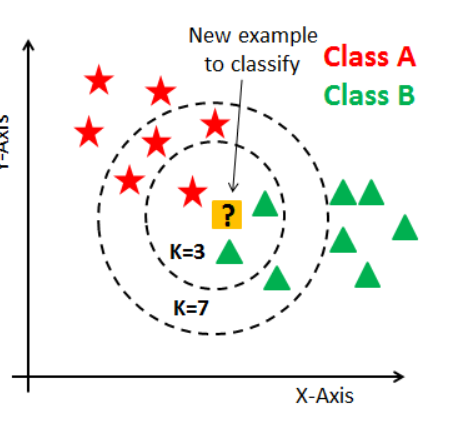
\includegraphics[width=9cm, keepaspectratio]{img/knn}
	\caption{Clasificador K-NN}\label{fig:knn}
\end{figure}


En la imagen  ~\ref{fig:knn} podemos ver como en este caso, las características serían dos, una en cada eje y por otro lado tendríamos tendríamos dos clases. En el caso de utilizar una K con valor tres, asignaría la entrada que estamos evaluando a la clase B, sin embargo, si tomamos el valor siete para la K, la clasificaría como clase A. Con este ejemplo, nos damos cuenta de que es importante que el valor de K sea pequeño. Este parámetro será uno de los que pueda modificar el usuario en la web de LearningML.


%%%%%%%%%%%%%%%%%%%%%%%%%%%%%%%%%%%%%%%%%%%%%%%%%%%%%%%%%%%%%%%%%%%%%%%%%%%%%%%%
%%%%%%%%%%%%%%%%%%%%%%%%%%%%%%%%%%%%%%%%%%%%%%%%%%%%%%%%%%%%%%%%%%%%%%%%%%%%%%%%
% DISEÑO E IMPLEMENTACIÓN %
%%%%%%%%%%%%%%%%%%%%%%%%%%%%%%%%%%%%%%%%%%%%%%%%%%%%%%%%%%%%%%%%%%%%%%%%%%%%%%%%

\cleardoublepage
\chapter{Diseño e implementación}

Aquí viene todo lo que has hecho tú (tecnológicamente). 
Puedes entrar hasta el detalle. 
Es la parte más importante de la memoria, porque describe lo que has hecho tú.
Eso sí, normalmente aconsejo no poner código, sino diagramas.

\section{Arquitectura antigua de LearningML} 
\label{sec:arquitecturaantigua}

Lo primero que hay que tener claro a la hora de hacer algún cambio en una aplicación web, es su estructura, por lo que vamos a ver como funcionaba la de LearningML antes de realizar el cambio en su forma de trabajar. Hay que tener en cuenta que LearningML está construido por Angular, por lo que esta compuesto por modulos, componentes y servicios. Es importante recordar que antes solo se usaba un algorítmo (redes neuronales) de ahí esta estructura. \\
Según esta construido LearningML, en el módulo principal \texttt{AppModule} se carga el componente \texttt{ml-model} y el componente \texttt{ml-test-model} uno para construir el modelo y otro para probarlo respectivamente. Estos dos componentes tienen importados a su vez los servicios \texttt{image-classifier} y \texttt{classifier}, uno para crear un modelo de imágenes y otro de texto. El servicio para clasificar texto se llama unicamente \texttt{classfier} porque fue el primero que se incorporó cuando Juanda creo la web y no sabía si se añadirían más en un futuro. \\
De manera transversal a todo esto tenemos el servicio \texttt{labeled-data-manager}, que es una especie de "cajón de sastre" donde se almacenan algunos datos que necesitamos en los otros servicios y componentes. 
Para la parte de test hay un solo componente llamado \texttt{ml-test-model} que llama a la función \texttt{classify} de \texttt{image-classifier} o a la función  \texttt{run} de \texttt{classifier}, dependiendo de si se estan clasificando imágenes o textos respectivamente.
Vamos a fijarnos en la figura ~\ref{fig:modeloantiguo} para ver que contiene cada uno de los servicios nombrados anteriormente.

\begin{figure}
	\centering
	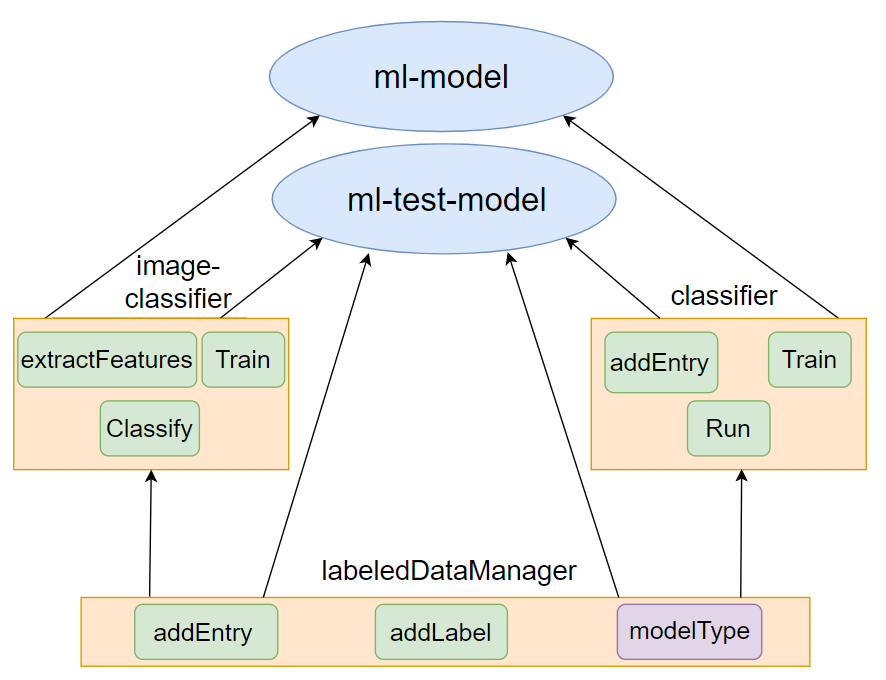
\includegraphics[width=12cm, keepaspectratio]{img/modeloantiguo}
	\caption{Estructura antigua de LearningML. En azul los componentes, en naranja los servicios, en verde las funciones y en morado las variables.}\label{fig:modeloantiguo}
\end{figure}


\begin{itemize}
  
	\item Labeled-Data-Manager: Es un servicio que se encarga de guardar los datos en bruto, ya sean imágenes o textos con la función \texttt{addEntry}. También almacena las etiquetas, es decir, las distintas posibles clases a las que puede pertenecer una entrada utilizando la función \texttt{addLabel}. Por último, guarda el tipo de modelo que se quiere construir directamente en la variable \texttt{modelType}. En caso de que carguemos los datos de un JSON, tambíen es aquí donde se realiza tanto la carga como la exportación.
 
	\item ImageClassifier: Dentro de este servicio encontramos tres funciones principales, \texttt{extractFeature} que se encarga de transformar las imágenes de entrada en tensores, \texttt{train} que construye el modelo y lo entrena y por último \texttt{classify} que evalua la imagen de entrada de test y la asgina a una de las posibles opciones (etiquetas). Dentro de esta última función tenemos que volver a llamar a \texttt{extractFeature} para que transforme la imágen a tensor y poder analizarla.

	\item Classifier: Este servicio lo que hace es transformar las entradas de texto en bruto en vectores, en esta ocasión se utiliza la librería BrainText, que es una adaptación que hizo Juanda de la librería Brain.js \footnote{\url{https://brain.js.org/}}. De nuevo, contiene la función \texttt{train} encargada de crear el modelo y entrenarlo y la función \texttt{run}, que sería el equivalente a la función  \texttt{classify} del punto anterior, es decir, lee el texto introducido, lo trata y lo evalúa y por último determina a cuál de los grupos o etiquetas pertenece.

\end{itemize}

\section{Arquitectura actual de LearningML} 
\label{sec:arquitecturaactual}

Como hemos visto en la sección anterior, tenemos tanto la extracción de características (el proceso de convertir los datos en bruto en un vector que pasar como entrada al constructor del modelo) como la construcción del modelo en el mismo servicio. La idea que tenemos en mente es que por un lado se extraigan las características y por otro lado se genere el modelo independientemente de si estamos clasificando imágenes o texto, ya que al constructor del modelo le entrara un vector sin importar si se ha construido de una forma u otra.\\
Ahora el componente \texttt{ml-model} importa los servicios de \texttt{feature-extraction} y \texttt{ml-algorithm}. Dentro de estos dos servicios, se importan a su vez en el primero \texttt{feature-extractor-image} y \texttt{feature-extractor-text} y en el segundo \texttt{ml-algorithm-image} y \texttt{ml-algorithm-text}.
En el componente \texttt{ml-model} existe la función \texttt{train}, la cual existia también antes pero llamaba directamente a uno de los dos antiguos servicios, ahora llama a \texttt{feature-extraction} y es este quién elige que servicio usar para extraer el vector dependiendo del tipo de dato. Después llama a \texttt{ml-algorithm} y este servicio decide que algorítmo utilizar para construir el modelo.\\
En la parte de prueba se ha dividido el componente \texttt{ml-test-model} en dos \texttt{ml-test-image} y \texttt{ml-test-text} para imágenes y texto respectivamente. El componente \texttt{ml-test-image} contiene la función \texttt{takeSnapshot} (en caso de que la imagen de prueba sea una foto a través de la cámara) y la función \texttt{onLoaded} (en caso de que la imagen sea un archivo ya existente), en ambos casos, se llama primero a \texttt{feature-extraction} y después a \texttt{ml-algorithm}. En el caso del texto funciona de la misma manera pero solo podemos introducir texto por teclado.\\
El servicio de \texttt{labeled-data-manager} sigue siendo transversal a todos los servicios y componentes, con el único añadido de que ahora guardamos el tipo de algorítmo que vamos a utilizar en la variable \texttt{mlAlgorithm}.
Esta estructura simplifica mucho las cosas y hace que el código sea más fácil de entender y de modificar en caso de que algún día haya que añadir nuevos tipos de datos o nuevos tipos de algorítmos. Hace que las funciones y en general el código sean similares para distintos tipo de datos, además, separa los dos problemas por completo haciendolos totalmente independientes uno de otro. De nuevo, vamos a ver la figura ~\ref{fig:modelonuevo} para entenderlo mejor.

\begin{figure}
	\centering
	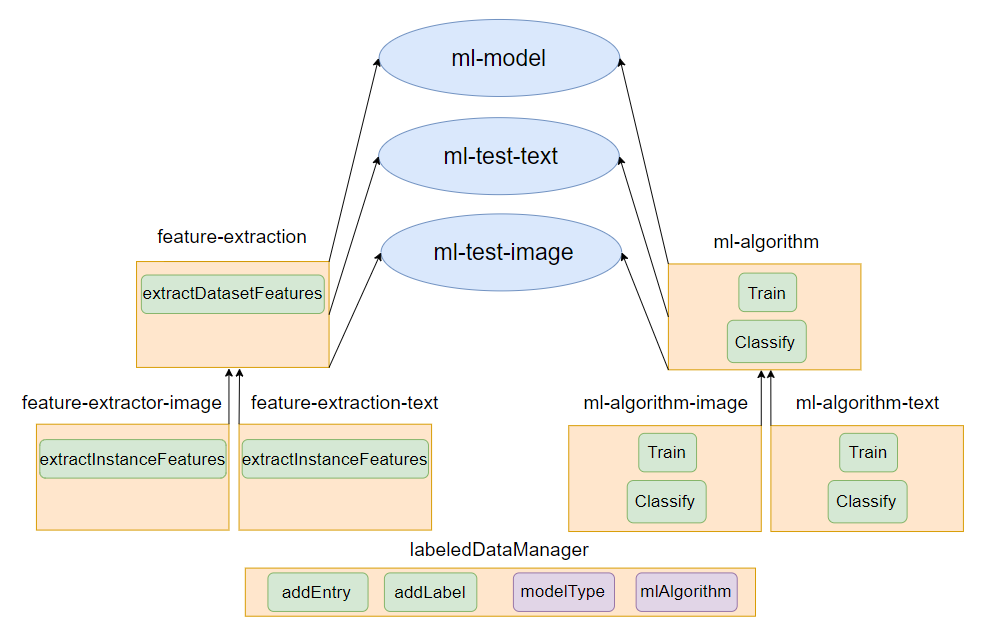
\includegraphics[width=12cm, keepaspectratio]{img/modelonuevo}
	\caption{Estructura nueva de LearningML. En azul los componentes, en naranja los servicios, en verde las funciones y en morado las variables.}\label{fig:modelonuevo}
\end{figure}

\begin{itemize}
  
	\item Labeled-Data-Manager: Este servicio como ya se ha comentado sigue siendo utilizado en todo el resto de servicios y componentes, con la diferencia de que ahora, además de los datos de etiquetas, datos en bruto de las entradas y tipo de modelo que ya guardaba antes, guarda también el tipo de algortimo en la variable \texttt{mlAlgorithm}.
 
	\item Feature-Extraction: En este servicio encontramos la función de \texttt{extractDatasetFeatures} que es la encargada de llamar a los otros dos servicios dependiendo de si se quieren extrar características de una imagen o de un texto.
\begin{itemize}
  
	\item Feature-Extractor-Image: Se encarga de extraer las características de las imágenes, es decir, de convertir la imagen en bruto a un tensor. La función que realmente hace esto de obtener el tensor dada una imagen es \texttt{extractInstanceFeatures}. Aunque tiene más funciones para por ejemplo construir un mapa con la etiqueta que corresponde a cada imagen.

	\item Feature-Extractor-Text: Se encarga de extraer las características de los textos, por tanto, con un texto como entrada obtenemos un tensor. De nuevo, para que la arquitectura tenga una estructura coherente, la función recibe el nombre de \texttt{extractInstanceFeatures}. 
\end{itemize}

	\item ml-Algorithm: Este servicio cuenta con dos funciones principales. \texttt{train} encargada de elegir a que sub-servicio llamar dependiendo del algorítmo que se quiere utilizar. Y la función \texttt{classify} que de nuevo, elige que sub-servicio utilizar en funcion del algorítmo.
\begin{itemize}
  
	\item ml-Algorithm-knn: Cuenta con dos funciones que son las que llama el servicio que esta por encima para entrenar (\texttt{train}) o evaluar  (\texttt{classify}) una entrada en el caso de que el algorítmo elegido por el usuario sea K-NN.

	\item ml-Algorithm-bayes: Cuenta con las mismas funciones que K-NN pero en este caso construye o evalua un clasificador utilizando el algorítmo de Naive Bayes.
\end{itemize}


\end{itemize}

Finalmente, recalcalcar que esta estructura si se utiliza correctamente permite añadir un nuevo tipo de dato o de clasificador únicamente creando los nuevos servicios. Debemos tener en cuenta que estos nuevos servicios para que encajen con lo que ya hay deben tener al menos las mismas funciones que los ya existentes, ya que son a las que llaman los servicios superiores. De esta manera, sin apenas tocar los servicios superiores (solo habría que añadir en el punto donde se elije el tipo de dato a extraer o el tipo de modelo, la opción de elegir lo nuevo que hayamos creado) podemos implementar nuevas funcionalidades en un futuro de manera más limpia y sencilla.



\section{Arquitectura general} 
\label{sec:arquitectura}

Si tu proyecto es un software, siempre es bueno poner la arquitectura (que es cómo se estructura tu programa a ``vista de pájaro'').



\section{Crear el clasificador de Naive Bayes} 
\label{sec:naivebayes}



\section{Crear el clasificador de K-NN} 
\label{sec:knn}



%%%%%%%%%%%%%%%%%%%%%%%%%%%%%%%%%%%%%%%%%%%%%%%%%%%%%%%%%%%%%%%%%%%%%%%%%%%%%%%%
%%%%%%%%%%%%%%%%%%%%%%%%%%%%%%%%%%%%%%%%%%%%%%%%%%%%%%%%%%%%%%%%%%%%%%%%%%%%%%%%
% EXPERIMENTOS Y VALIDACIÓN %
%%%%%%%%%%%%%%%%%%%%%%%%%%%%%%%%%%%%%%%%%%%%%%%%%%%%%%%%%%%%%%%%%%%%%%%%%%%%%%%%

\cleardoublepage
\chapter{Experimentos y validación}

Este capítulo se introdujo como requisito en 2019. 
Describe los experimentos y casos de test que tuviste que implementar para validar tus resultados. 
Incluye también los resultados de validación que permiten afirmar que tus resultados son correctos. 

\section{Prueba del clasificador de Naive Bayes} 
\label{sec:pruebabayes}

\section{Prueba del clasificador de K-NN} 
\label{sec:pruebaknn}

%%%%%%%%%%%%%%%%%%%%%%%%%%%%%%%%%%%%%%%%%%%%%%%%%%%%%%%%%%%%%%%%%%%%%%%%%%%%%%%%
%%%%%%%%%%%%%%%%%%%%%%%%%%%%%%%%%%%%%%%%%%%%%%%%%%%%%%%%%%%%%%%%%%%%%%%%%%%%%%%%
% RESULTADOS %
%%%%%%%%%%%%%%%%%%%%%%%%%%%%%%%%%%%%%%%%%%%%%%%%%%%%%%%%%%%%%%%%%%%%%%%%%%%%%%%%

%\cleardoublepage
%\chapter{Resultados}

%En este capítulo se incluyen los resultados de tu trabajo fin de grado.

%Si es una herramienta de análisis lo que has realizado, aquí puedes poner ejemplos de haberla utilizado para que se vea su utilidad.


%%%%%%%%%%%%%%%%%%%%%%%%%%%%%%%%%%%%%%%%%%%%%%%%%%%%%%%%%%%%%%%%%%%%%%%%%%%%%%%%
%%%%%%%%%%%%%%%%%%%%%%%%%%%%%%%%%%%%%%%%%%%%%%%%%%%%%%%%%%%%%%%%%%%%%%%%%%%%%%%%
% CONCLUSIONES %
%%%%%%%%%%%%%%%%%%%%%%%%%%%%%%%%%%%%%%%%%%%%%%%%%%%%%%%%%%%%%%%%%%%%%%%%%%%%%%%%

\cleardoublepage
\chapter{Conclusiones}
\label{chap:conclusiones}


\section{Consecución de objetivos}
\label{sec:consecucion-objetivos}

Esta sección es la sección espejo de las dos primeras del capítulo de objetivos, donde se planteaba el objetivo general y se elaboraban los específicos.

Es aquí donde hay que debatir qué se ha conseguido y qué no. 
Cuando algo no se ha conseguido, se ha de justificar, en términos de qué problemas se han encontrado y qué medidas se han tomado para mitigar esos problemas.

Y si has llegado hasta aquí, siempre es bueno pasarle el corrector ortográfico, que las erratas quedan fatal en la memoria final.
Para eso, en Linux tenemos aspell, que se ejecuta de la siguiente manera desde la línea de \emph{shell}:

\begin{verbatim}
  aspell --lang=es_ES -c memoria.tex
\end{verbatim}

\section{Aplicación de lo aprendido}
\label{sec:aplicacion}

Aquí viene lo que has aprendido durante el Grado/Máster y que has aplicado en el TFG/TFM. Una buena idea es poner las asignaturas más relacionadas y comentar en un párrafo los conocimientos y habilidades puestos en práctica.

\begin{enumerate}
  \item a
  \item b
\end{enumerate}


\section{Lecciones aprendidas}
\label{sec:lecciones_aprendidas}

Aquí viene lo que has aprendido en el Trabajo Fin de Grado.

\begin{enumerate}
  \item dd
  \item Aquí viene otro.
\end{enumerate}


\section{Trabajos futuros}
\label{sec:trabajos_futuros}

Ningún proyecto ni software se termina, así que aquí vienen ideas y funcionalidades que estaría bien tener implementadas en el futuro.

Es un apartado que sirve para dar ideas de cara a futuros TFGs/TFMs.


%%%%%%%%%%%%%%%%%%%%%%%%%%%%%%%%%%%%%%%%%%%%%%%%%%%%%%%%%%%%%%%%%%%%%%%%%%%%%%%%
%%%%%%%%%%%%%%%%%%%%%%%%%%%%%%%%%%%%%%%%%%%%%%%%%%%%%%%%%%%%%%%%%%%%%%%%%%%%%%%%
% APÉNDICE(S) %
%%%%%%%%%%%%%%%%%%%%%%%%%%%%%%%%%%%%%%%%%%%%%%%%%%%%%%%%%%%%%%%%%%%%%%%%%%%%%%%%

\cleardoublepage
\appendix
\chapter{Manual de usuario}
\label{app:manual}

Esto es un apéndice.
Si has creado una aplicación, siempre viene bien tener un manual de usuario.
Pues ponlo aquí.

%%%%%%%%%%%%%%%%%%%%%%%%%%%%%%%%%%%%%%%%%%%%%%%%%%%%%%%%%%%%%%%%%%%%%%%%%%%%%%%%
%%%%%%%%%%%%%%%%%%%%%%%%%%%%%%%%%%%%%%%%%%%%%%%%%%%%%%%%%%%%%%%%%%%%%%%%%%%%%%%%
% BIBLIOGRAFIA %
%%%%%%%%%%%%%%%%%%%%%%%%%%%%%%%%%%%%%%%%%%%%%%%%%%%%%%%%%%%%%%%%%%%%%%%%%%%%%%%%

\cleardoublepage

% Las siguientes dos instrucciones es todo lo que necesitas
% para incluir las citas en la memoria
\bibliographystyle{abbrv}
\bibliography{memoria}  % memoria.bib es el nombre del fichero que contiene
% las referencias bibliográficas. Abre ese fichero y mira el formato que tiene,
% que se conoce como BibTeX. Hay muchos sitios que exportan referencias en
% formato BibTeX. Prueba a buscar en http://scholar.google.com por referencias
% y verás que lo puedes hacer de manera sencilla.
% Más información: 
% http://texblog.org/2014/04/22/using-google-scholar-to-download-bibtex-citations/

\end{document}
